\documentclass[11pt,a4paper]{article}
\usepackage[margin=1in]{geometry}
\usepackage{graphicx}
\usepackage{amsmath}
\usepackage{amssymb}
\usepackage{hyperref}
\usepackage{float}
\usepackage{subcaption}

\title{COL7(6)83 Assignment 4 \\ Morphological Operations, Edge Detection, and Segmentation}

\begin{document}

\maketitle

\section{Problem 1: Text Character Detection using Binary Morphology}

\subsection{Overview}
This problem explores binary morphological operations for detecting specific characters in scanned text documents. Starting with a thresholded binary image of printed text, we progressively refine our detection strategy to identify all instances of the lowercase letter "c" while avoiding false positives from similar characters.

The input image $A$ is a binary representation where text pixels have value 1 and background pixels have value 0. A manually cropped lowercase "c" serves as the initial structuring element $B$.

\subsection{Part (a): Basic Morphological Operations}

\subsubsection{Implementation}
Binary erosion and dilation form the foundation of mathematical morphology. For a binary image $A$ and structuring element $B$, these operations are defined as:

\textbf{Dilation:}
$$(A \oplus B)(i,j) = \bigvee_{(s,t) \in B} A(i+s, j+t)$$

The dilation operation places the structuring element at each foreground pixel in $A$ and marks all positions covered by $B$ as foreground in the output. This effectively expands the foreground regions.

\textbf{Erosion:}
$$(A \ominus B)(i,j) = \bigwedge_{(s,t) \in B} A(i+s, j+t)$$

The erosion operation places the structuring element at each position and marks the center as foreground only if $B$ fits entirely within the foreground of $A$. This shrinks foreground regions.

\textbf{Closing:}
$$A \bullet B = (A \oplus B) \ominus B$$

Closing performs dilation followed by erosion, which fills small gaps and connects nearby components while approximately preserving their size.

\subsubsection{Results}
We demonstrate dilation and closing on the text image $A$ using a disk-shaped structuring element with radius $r = 2$ pixels. The disk is defined as:
$$\text{disk}(r) = \{(x,y) : x^2 + y^2 \leq r^2\}$$

\begin{figure}[H]
\centering
\begin{subfigure}[b]{0.45\textwidth}
    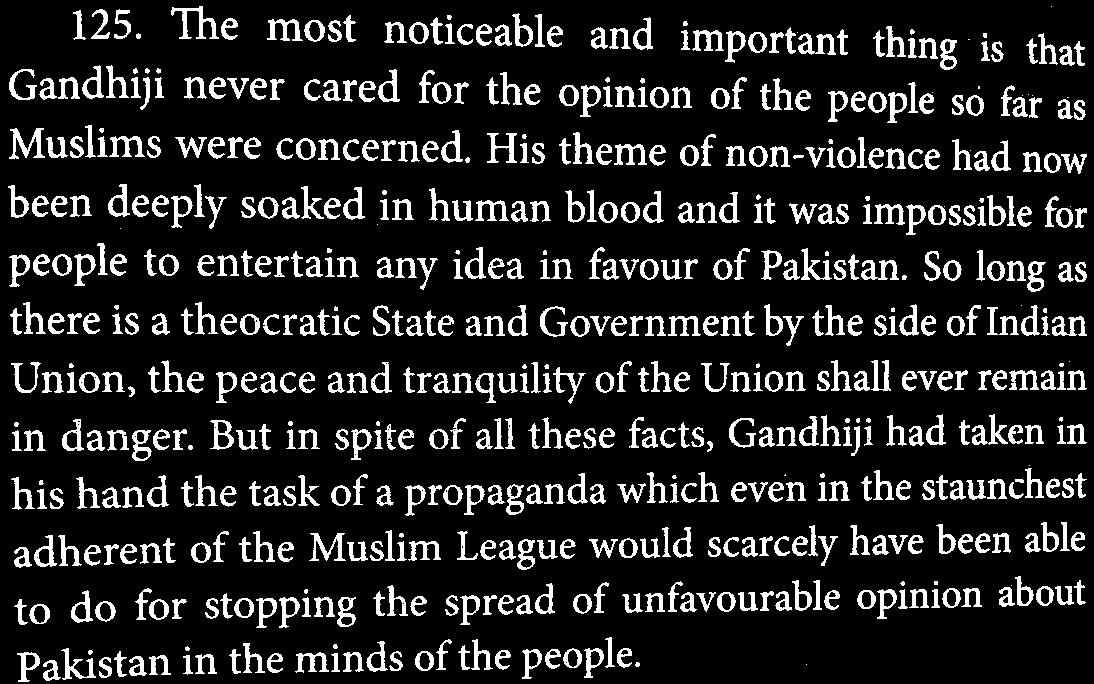
\includegraphics[width=\textwidth]{part1/results/1a_original.png}
    \caption{Original binary image $A$}
\end{subfigure}
\hfill
\begin{subfigure}[b]{0.45\textwidth}
    
\includegraphics[width=\textwidth]{part1/results/1a_disk_se.png}
    \caption{Disk structuring element (radius 2)}
\end{subfigure}
\caption{Input image and structuring element}
\end{figure}

\begin{figure}[H]
\centering
\begin{subfigure}[b]{0.45\textwidth}
    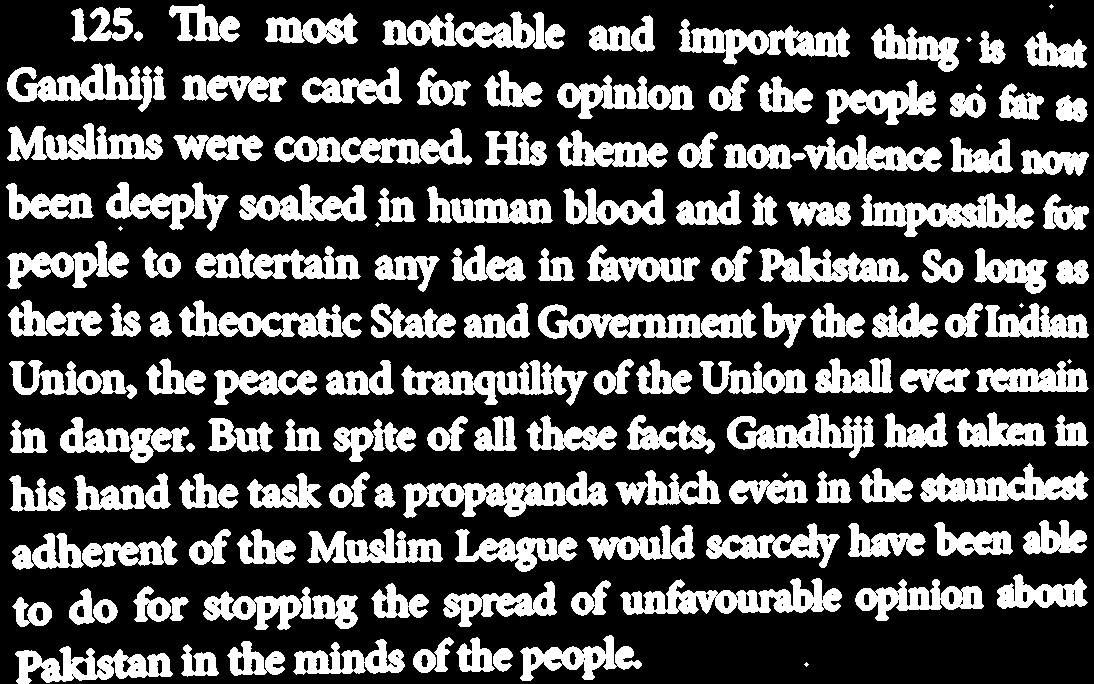
\includegraphics[width=\textwidth]{part1/results/1a_dilated.png}
    \caption{$A \oplus B$ (dilation)}
\end{subfigure}
\hfill
\begin{subfigure}[b]{0.45\textwidth}
    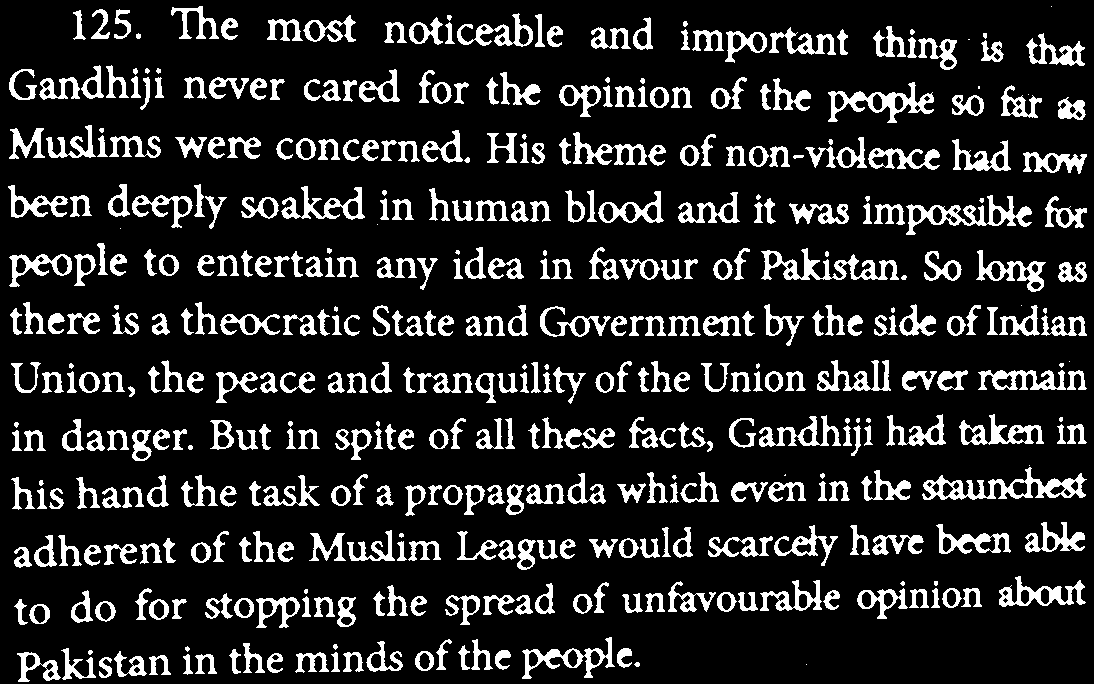
\includegraphics[width=\textwidth]{part1/results/1a_closed.png}
    \caption{$A \bullet B$ (closing)}
\end{subfigure}
\caption{Results of dilation and closing operations}
\end{figure}

The dilation expands all text strokes uniformly, making thin letters thicker. The closing operation fills small gaps within and between characters, bridging broken strokes while maintaining overall character structure.

\subsection{Part (b): Initial Character Detection via Opening}

\subsubsection{Method}
To detect occurrences of the letter "c", we use morphological opening:
$$A \circ B = (A \ominus B) \oplus B$$

Opening performs erosion followed by dilation. The erosion removes all regions where $B$ does not fit, leaving only locations that match the shape of $B$. The subsequent dilation restores the remaining regions to approximately their original size.

For character detection, opening identifies locations where the structuring element $B$ (the template "c") fits within the image $A$. Pixels that survive the erosion-dilation sequence indicate potential matches.

\subsubsection{Results and Discussion}

\begin{figure}[H]
\centering
\begin{subfigure}[b]{0.45\textwidth}
    
\includegraphics[width=\textwidth]{part1/results/1b_opening.png}
    \caption{Opening result $A \circ B$}
\end{subfigure}
\hfill
\begin{subfigure}[b]{0.45\textwidth}
    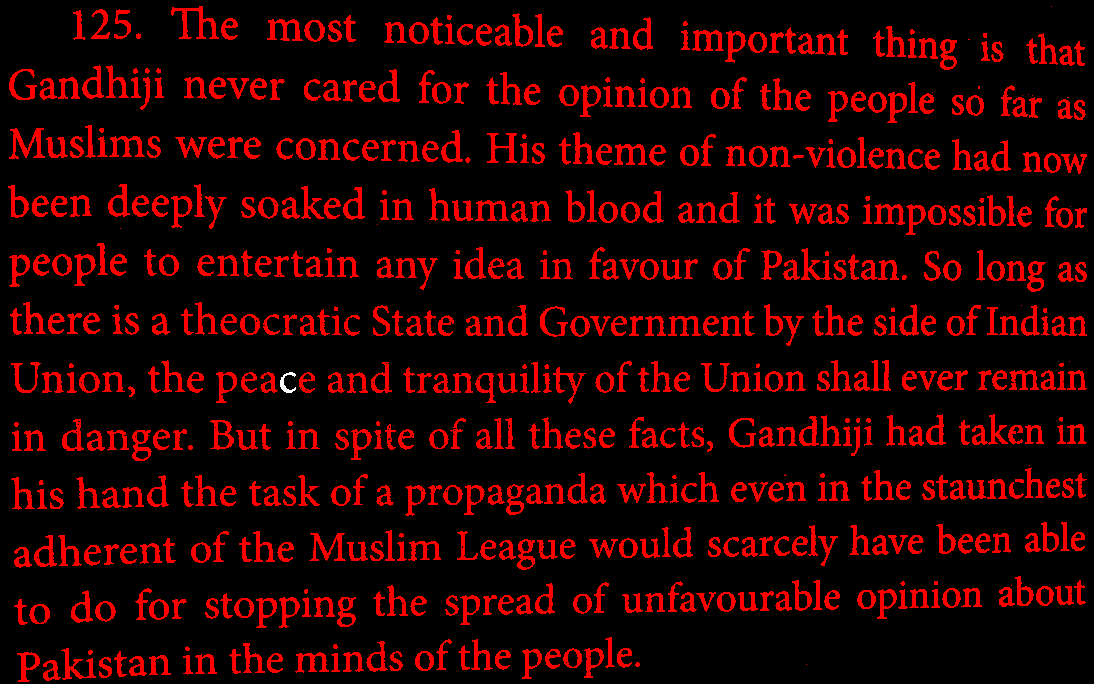
\includegraphics[width=\textwidth]{part1/results/1b_opening_rgb.png}
    \caption{RGB visualization (detected: white, undetected: red)}
\end{subfigure}
\caption{Part (b): Character detection using the original structuring element}
\end{figure}

The RGB visualization displays detected letters in white (all color channels active) and undetected letters in red (only red channel active). This clearly shows which instances of "c" were successfully identified.

\textbf{Why not all c's were found:} The opening operation is highly sensitive to exact shape matching. Several factors cause missed detections:

\begin{itemize}
    \item \textbf{Font variations:} Even within the same font, individual character instances may have slight rendering differences due to anti-aliasing, printing artifacts, or scanning noise.
    \item \textbf{Size variations:} Small differences in character size prevent perfect alignment between $B$ and target characters.
    \item \textbf{Stroke width variations:} Inconsistent ink density during printing or thresholding creates characters with varying stroke widths.
    \item \textbf{Structural requirements:} The erosion step requires $B$ to fit completely within the foreground. Any pixel mismatch causes the entire character to be rejected.
\end{itemize}

The strict geometric requirements of erosion make opening unsuitable for robust character detection when exact pixel-perfect matching cannot be guaranteed.

\subsection{Part (c): Improved Detection with Modified Structuring Element}

\subsubsection{Strategy}
To detect all instances of "c", we must relax the strict geometric constraints while maintaining shape selectivity. The key insight is that the defining characteristic of "c" is its overall shape, not its exact pixel configuration.

We create a modified structuring element $B_1$ by eroding the original $B$ with a small disk:
$$B_1 = B \ominus \text{disk}(1) \ominus \text{disk}(1)$$

The double erosion with unit disks shrinks $B$ uniformly, reducing it to its "core" shape. This smaller structuring element is more tolerant to minor variations in character rendering.

\subsubsection{Mathematical Rationale}
The erosion process removes the boundary pixels of $B$, creating a smaller template that captures the essential topology of "c" without requiring exact boundary matching. This can be understood through the property:
$$(A \ominus B_1) \supseteq (A \ominus B)$$

Since $B_1 \subset B$, the smaller structuring element fits more easily, detecting a superset of the original matches. The trade-off is that $B_1$ may also match other letters with similar core shapes, such as "e".

\subsubsection{Results}

\begin{figure}[H]
\centering
\begin{subfigure}[b]{0.3\textwidth}
    
\includegraphics[width=\textwidth]{part1/results/1c_b_original.png}
    \caption{Original $B$}
\end{subfigure}
\hfill
\begin{subfigure}[b]{0.3\textwidth}
    
\includegraphics[width=\textwidth]{part1/results/1c_b1_eroded.png}
    \caption{Eroded $B_1$}
\end{subfigure}
\hfill
\begin{subfigure}[b]{0.3\textwidth}
    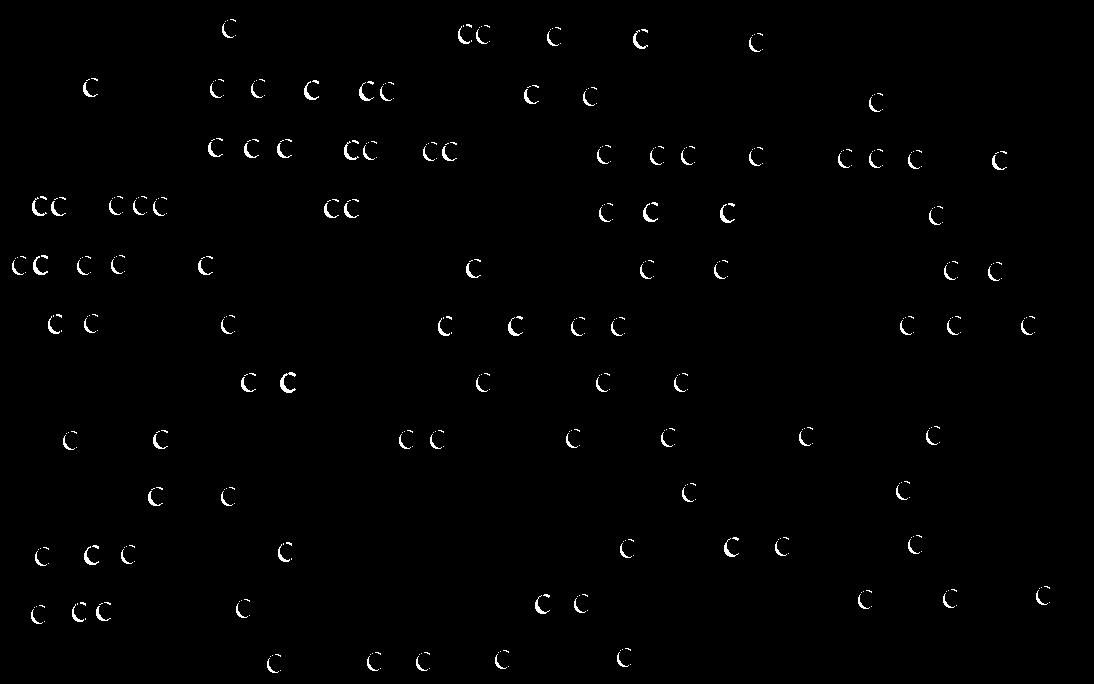
\includegraphics[width=\textwidth]{part1/results/1c_opening_b1.png}
    \caption{Opening $A \circ B_1$}
\end{subfigure}
\caption{Modified structuring element and detection results}
\end{figure}

\begin{figure}[H]
\centering

\includegraphics[width=0.7\textwidth]{part1/results/1c_opening_b1_rgb.png}
\caption{RGB visualization showing improved detection (all c's detected in white)}
\end{figure}

The modified structuring element $B_1$ successfully detects all instances of "c" in the text. However, as predicted, it also detects some lowercase "e" characters, which share a similar core shape (a curved body with an opening on the right side). This demonstrates the fundamental trade-off in template matching: reducing selectivity to improve recall (finding all true positives) inevitably increases false positives.

\subsection{Part (d): Precise Detection via Hit-or-Miss Transform}

\subsubsection{Theory}
To eliminate false positives while maintaining complete detection, we employ the hit-or-miss transform, which tests for both the presence and absence of specific features. Given two structuring elements $B_1$ (hit template) and $B_2$ (miss template), the transform is defined as:
$$A \circledast (B_1, B_2) = (A \ominus B_1) \cap (A^c \ominus B_2)$$

where $A^c$ denotes the complement of $A$. This operation identifies locations where:
\begin{enumerate}
    \item The foreground structure matches $B_1$ (the "hit" condition)
    \item The background structure matches $B_2$ (the "miss" condition)
\end{enumerate}

\subsubsection{Constructing the Miss Template}
The key to distinguishing "c" from "e" lies in the gap region. In a lowercase "c", the right side is open with no horizontal bar crossing the middle. In contrast, "e" has a horizontal stroke in this region.

We construct $B_2$ to detect background pixels in the region where "e" would have its horizontal crossbar:
$$B_2 = \text{rectangular region} \times \text{disk}(1)$$

The rectangular region spans the middle height of the character and extends into the right-side opening. The dilation by a small disk provides tolerance for minor position variations.

\subsubsection{Implementation Details}
The complete detection procedure:
\begin{enumerate}
    \item Erode $A$ with $B_1$ to find locations matching the core "c" shape
    \item Erode $A^c$ (background) with $B_2$ to find locations with the required background pattern
    \item Intersect these results to obtain points satisfying both conditions
    \item Dilate the detected points with the original $B$ to reconstruct full character shapes
\end{enumerate}

The final dilation step is crucial for visualization, as the hit-or-miss transform outputs only single marker points rather than full character shapes.

\subsubsection{Results}

\begin{figure}[H]
\centering
\begin{subfigure}[b]{0.3\textwidth}
    
\includegraphics[width=\textwidth]{part1/results/1d_b2_miss.png}
    \caption{Miss template $B_2$}
\end{subfigure}
\hfill
\begin{subfigure}[b]{0.3\textwidth}
    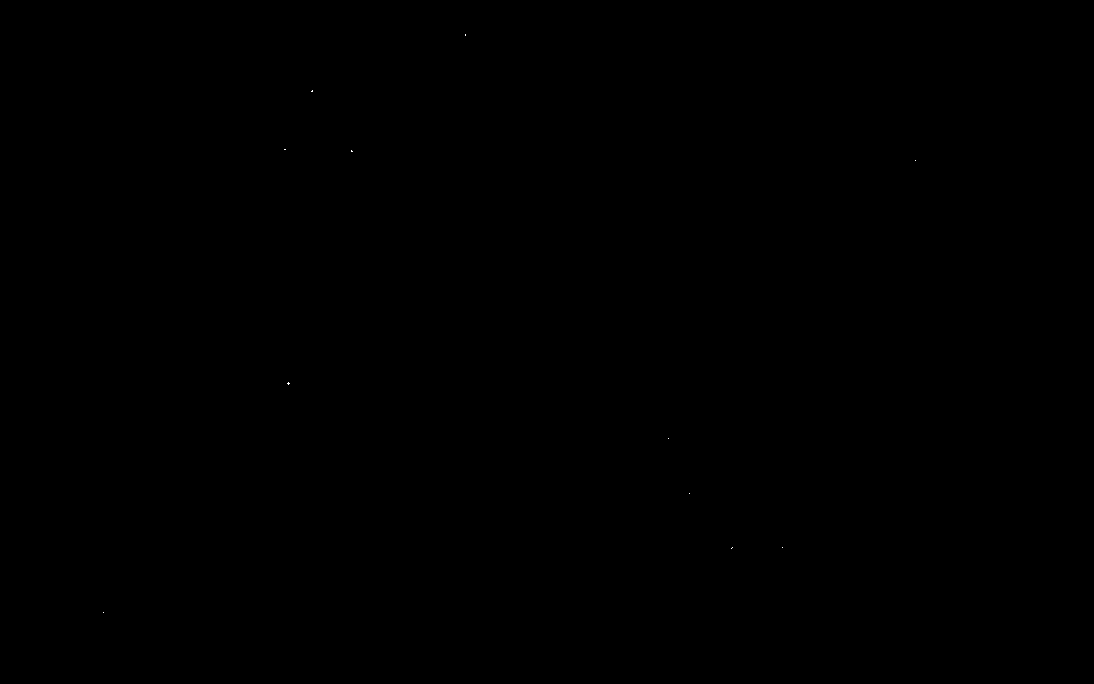
\includegraphics[width=\textwidth]{part1/results/1d_hmt_points.png}
    \caption{Hit-or-miss result (marker points)}
\end{subfigure}
\hfill
\begin{subfigure}[b]{0.3\textwidth}
    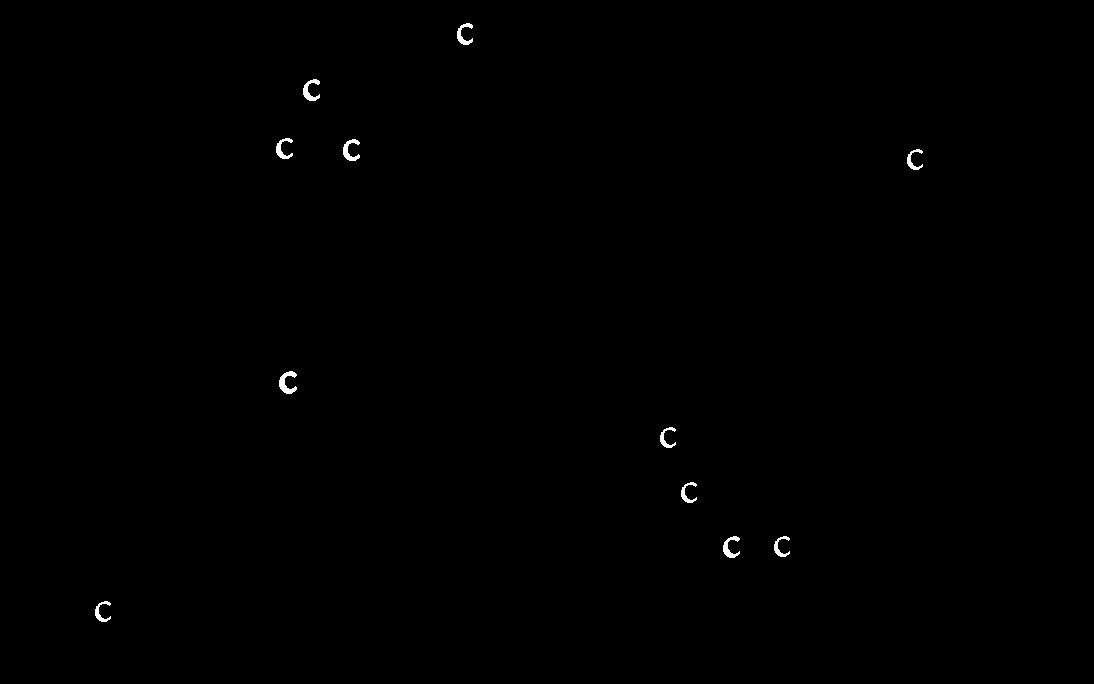
\includegraphics[width=\textwidth]{part1/results/1d_detected.png}
    \caption{Reconstructed detections}
\end{subfigure}
\caption{Hit-or-miss transform for precise "c" detection}
\end{figure}

\begin{figure}[H]
\centering

\includegraphics[width=0.7\textwidth]{part1/results/1d_detected_rgb.png}
\caption{Final RGB visualization showing only "c" characters detected (white)}
\end{figure}

The hit-or-miss transform successfully identifies all instances of "c" while rejecting "e" characters. The miss template $B_2$ ensures that only characters with an open right side are detected. The marker points from the transform are then dilated by the original structuring element $B$ to visualize the complete character shapes.

This approach demonstrates the power of morphological methods for shape-based pattern recognition: by combining positive (hit) and negative (miss) constraints, we achieve both high recall (finding all targets) and high precision (avoiding false positives).

\newpage
\section{Problem 2: Blood Vessel Analysis in Fundus Images}

\subsection{Overview}
Fundus photography captures the interior surface of the eye, revealing the retinal blood vessel network. Analyzing vessel structure is crucial for diagnosing various ocular and systemic diseases. This problem develops a morphological pipeline to extract vessels from a fundus image and characterize their thickness distribution.

\subsection{Part (a): Grayscale Morphological Operations}

\subsubsection{Implementation}
Grayscale morphology extends binary operations to intensity images. For a grayscale image $f$ and flat structuring element $B$, the operations are defined using supremum and infimum:

\textbf{Grayscale Erosion:}
$$(f \ominus B)(x,y) = \min_{(s,t) \in B} f(x+s, y+t)$$

At each position, erosion selects the minimum intensity within the structuring element's neighborhood. This darkens bright regions and removes small bright features.

\textbf{Grayscale Dilation:}
$$(f \oplus B)(x,y) = \max_{(s,t) \in B} f(x+s, y+t)$$

Dilation selects the maximum intensity, brightening dark regions and removing small dark features.

\textbf{Opening and Closing:}
$$f \circ B = (f \ominus B) \oplus B$$
$$f \bullet B = (f \oplus B) \ominus B$$

Opening removes bright features smaller than $B$, while closing removes dark features smaller than $B$.

\subsubsection{Results}

\begin{figure}[H]
\centering
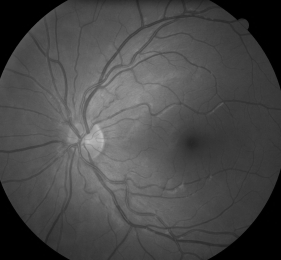
\includegraphics[width=0.5\textwidth]{part2/results/2_original.png}
\caption{Original fundus image (grayscale conversion)}
\end{figure}

\begin{figure}[H]
\centering
\begin{subfigure}[b]{0.45\textwidth}
    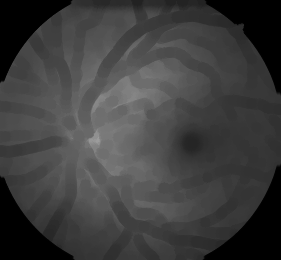
\includegraphics[width=\textwidth]{part2/results/2a_eroded.png}
    \caption{Erosion $f \ominus B$}
\end{subfigure}
\hfill
\begin{subfigure}[b]{0.45\textwidth}
    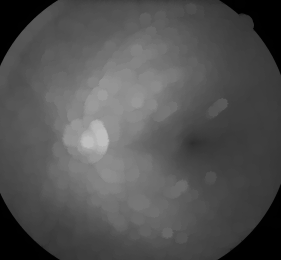
\includegraphics[width=\textwidth]{part2/results/2a_dilated.png}
    \caption{Dilation $f \oplus B$}
\end{subfigure}
\end{figure}

\begin{figure}[H]
\centering
\begin{subfigure}[b]{0.45\textwidth}
    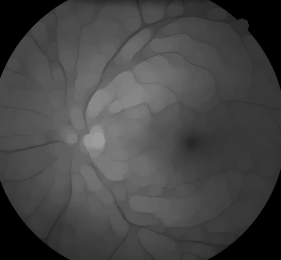
\includegraphics[width=\textwidth]{part2/results/2a_opened.png}
    \caption{Opening $f \circ B$}
\end{subfigure}
\hfill
\begin{subfigure}[b]{0.45\textwidth}
    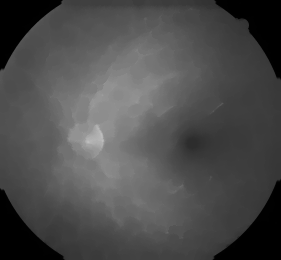
\includegraphics[width=\textwidth]{part2/results/2a_closed.png}
    \caption{Closing $f \bullet B$}
\end{subfigure}
\caption{Four basic grayscale morphological operations (disk SE, radius 5)}
\end{figure}

Erosion darkens the image by selecting local minima, making vessels more prominent against the lighter background. Dilation brightens by selecting local maxima, reducing vessel visibility. Opening removes small bright structures while closing removes small dark structures, both smoothing the image at the scale defined by $B$.

\subsection{Part (b): Vessel Extraction via Bottom-Hat Transform}

\subsubsection{Method}
Blood vessels appear as dark, elongated structures against a brighter background with slowly varying intensity. The bottom-hat transform isolates such features by computing:
$$\text{BH}(f) = (f \bullet B) - f$$

This measures how much darker each pixel is compared to its local neighborhood, as determined by the closing operation. The closing $f \bullet B$ fills dark features smaller than $B$, creating a smoothed image. Subtracting the original from this gives positive values where $f$ was darker than its surroundings.

\subsubsection{Structuring Element Selection}
The critical parameter is the disk radius $r$. The structuring element must be:
\begin{itemize}
    \item Large enough to span the widest vessels, ensuring they are removed by closing
    \item Large enough to smooth over intensity variations in the background
    \item Small enough that vessels remain darker than the closed image
\end{itemize}

Through experimentation, $r = 12$ pixels was found to effectively capture vessels of varying sizes while suppressing background variation.

\subsubsection{Results}

\begin{figure}[H]
\centering
\begin{subfigure}[b]{0.45\textwidth}
    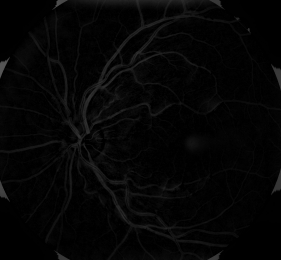
\includegraphics[width=\textwidth]{part2/results/2b_bottom_hat_raw.png}
    \caption{Raw bottom-hat output}
\end{subfigure}
\hfill
\begin{subfigure}[b]{0.45\textwidth}
    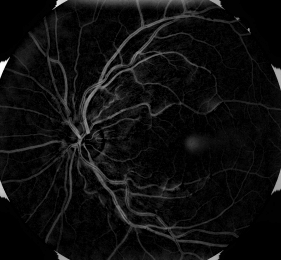
\includegraphics[width=\textwidth]{part2/results/2b_vessels.png}
    \caption{Contrast-stretched vessels}
\end{subfigure}
\caption{Bottom-hat transform for vessel extraction (radius 12)}
\end{figure}

The bottom-hat transform successfully extracts the vessel network. Contrast stretching to the full [0, 255] range enhances visibility. The fine vessel structure is well-preserved, though some vessels exhibit dark gaps where specular reflections occur.

\subsection{Part (c): Gap Filling via Grayscale Closing}

\subsubsection{Problem Analysis}
The bright highlights in some vessels are caused by specular reflection from blood vessel walls. In the bottom-hat image, these appear as dark gaps interrupting vessel continuity. These gaps will cause thickness estimation algorithms to underestimate vessel diameter by treating a single vessel as multiple disconnected segments.

\subsubsection{Solution}
To fill these gaps, we apply grayscale closing with a small disk structuring element:
$$f_{\text{filled}} = f_{\text{vessels}} \bullet B_{\text{small}}$$

The closing operation fills dark features smaller than the structuring element. By choosing a small radius ($r = 2$ pixels), we specifically target the narrow gaps while minimizing impact on the overall vessel structure.

\subsubsection{Theoretical Justification}
Closing satisfies the important property of being an increasing transformation:
$$f_1 \leq f_2 \implies (f_1 \bullet B) \leq (f_2 \bullet B)$$

This ensures that closing never creates new dark regions; it can only fill or preserve existing dark features. The effect is localized to pixels within distance $r$ of bright regions, limiting unintended modifications to vessel structure.

\subsubsection{Results}

\begin{figure}[H]
\centering
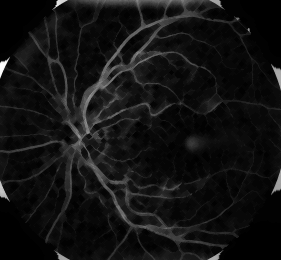
\includegraphics[width=0.6\textwidth]{part2/results/2c_vessels_filled.png}
\caption{Vessels after gap filling (closing with radius 2)}
\end{figure}

The closing operation successfully bridges the dark gaps within vessels, creating continuous structures suitable for thickness analysis. The small structuring element preserves fine vessel details while eliminating reflection artifacts.

\subsection{Part (d): Thickness Distribution via Granulometry}

\subsubsection{Granulometry Theory}
Granulometry is a morphological technique for characterizing the size distribution of structures in an image. The method is based on the observation that opening with a structuring element of size $r$ removes all connected components smaller than $r$.

For vessel analysis, we compute a size spectrum by measuring the area of remaining vessel pixels after opening with disks of increasing radius:
$$A(r) = \sum_{(x,y)} \left[(f_{\text{binary}} \circ B_r)(x,y)\right]$$

where $f_{\text{binary}}$ is a thresholded binary vessel image and $B_r$ is a disk of radius $r$.

\subsubsection{Pattern Spectrum}
The pattern spectrum, or size distribution, is the derivative of $A(r)$:
$$D(r) = A(r) - A(r+1)$$

This measures the area removed by increasing the structuring element size from $r$ to $r+1$. Peaks in $D(r)$ indicate common vessel widths in the image, as many vessels disappear when the opening structuring element exceeds their diameter.

\subsubsection{Implementation}
The analysis procedure:
\begin{enumerate}
    \item Threshold the gap-filled vessel image to create a binary mask
    \item For each radius $r \in \{1, 2, \ldots, 15\}$:
    \begin{itemize}
        \item Construct disk structuring element $B_r$
        \item Compute opening $f_{\text{binary}} \circ B_r$
        \item Count remaining foreground pixels $A(r)$
    \end{itemize}
    \item Compute differences $D(r) = A(r) - A(r+1)$
    \item Plot both $A(r)$ and $D(r)$ for analysis
\end{enumerate}

\subsubsection{Results}

\begin{figure}[H]
\centering
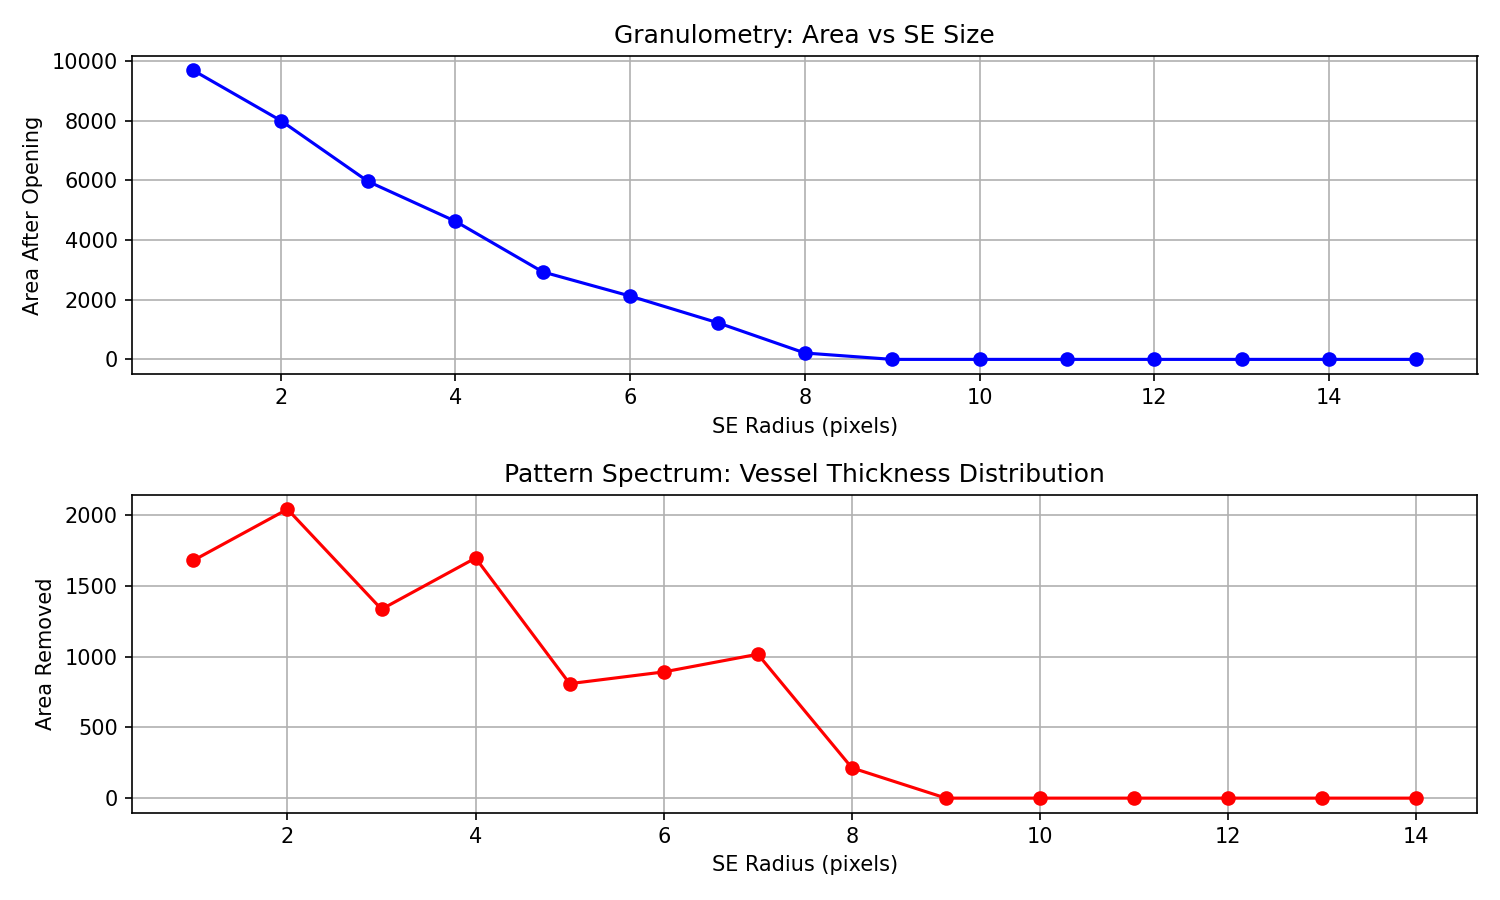
\includegraphics[width=0.85\textwidth]{part2/results/2d_granulometry.png}
\caption{Granulometry analysis: area curve and pattern spectrum}
\end{figure}

\textbf{Interpretation:}

The area curve $A(r)$ shows monotonic decrease, as larger openings remove more vessel pixels. The steep initial decline indicates many thin vessels, while the gradual tail suggests some thick vessels persist to larger radii.

The pattern spectrum $D(r)$ reveals the thickness distribution:
\begin{itemize}
    \item \textbf{Peak at $r = 2$-$3$ pixels:} The majority of vessels have small diameter, corresponding to capillaries and small arterioles/venules
    \item \textbf{Secondary elevation at $r = 5$-$7$ pixels:} Medium-sized vessels, likely representing primary retinal vessels
    \item \textbf{Extended tail to $r = 12$-$15$ pixels:} A few large vessels, probably the main retinal arteries and veins
\end{itemize}

This distribution is consistent with the hierarchical structure of retinal vasculature, where numerous small vessels branch from fewer large vessels. The granulometry technique successfully characterizes this multi-scale organization using purely morphological operations.

\newpage
\section{Problem 3: Straight Line Detection in Building Images}

\subsection{Overview}
Detecting straight edges and their intersections in building photographs is fundamental to architectural analysis and 3D reconstruction. This problem implements a complete edge-to-line pipeline: Canny edge detection to identify edge pixels, followed by the Hough transform to extract straight line parameters.

\subsection{Part (a): Canny Edge Detection}

\subsubsection{Algorithm Overview}
The Canny edge detector is a multi-stage algorithm designed to find edges with good localization and minimal false detections. The five stages are:

\begin{enumerate}
    \item \textbf{Gaussian smoothing:} Reduce noise via convolution with Gaussian kernel
    \item \textbf{Gradient computation:} Calculate magnitude and direction using Sobel operators
    \item \textbf{Non-maximum suppression:} Thin edges to single-pixel width
    \item \textbf{Double thresholding:} Classify edges as strong, weak, or non-edge
    \item \textbf{Edge tracking by hysteresis:} Connect weak edges to strong edges
\end{enumerate}

\subsubsection{Stage 1: Gaussian Smoothing}
Edges are susceptible to noise, as intensity derivatives amplify high-frequency variations. Gaussian smoothing provides optimal noise reduction in a least-squares sense. The kernel is:
$$G(x,y;\sigma) = \frac{1}{2\pi\sigma^2}\exp\left(-\frac{x^2+y^2}{2\sigma^2}\right)$$

The parameter $\sigma$ controls the amount of smoothing. Larger $\sigma$ removes more noise but also blurs true edges. The kernel size is chosen as $\lceil 6\sigma \rceil$ to capture 99.7\% of the Gaussian mass.

For this implementation, $\sigma = 1.5$ pixels provides a balance between noise suppression and edge preservation for building photographs.

\subsubsection{Stage 2: Gradient Computation}
The gradient indicates edge strength and orientation. We use Sobel operators for discrete differentiation:
$$S_x = \begin{bmatrix} -1 & 0 & 1 \\ -2 & 0 & 2 \\ -1 & 0 & 1 \end{bmatrix}, \quad S_y = \begin{bmatrix} -1 & -2 & -1 \\ 0 & 0 & 0 \\ 1 & 2 & 1 \end{bmatrix}$$

These kernels approximate $\frac{\partial f}{\partial x}$ and $\frac{\partial f}{\partial y}$ while providing some smoothing perpendicular to the derivative direction. The gradient magnitude and direction are:
$$|\nabla f| = \sqrt{G_x^2 + G_y^2}, \quad \theta = \arctan\left(\frac{G_y}{G_x}\right)$$

where $G_x = f * S_x$ and $G_y = f * S_y$.

\subsubsection{Stage 3: Non-Maximum Suppression}
Gradient magnitude produces thick edges where intensity changes gradually. Non-maximum suppression (NMS) thins these to single-pixel width by suppressing pixels that are not local maxima along the gradient direction.

For each pixel $(x,y)$, we:
\begin{enumerate}
    \item Quantize gradient direction $\theta(x,y)$ to the nearest 45° increment (0°, 45°, 90°, 135°)
    \item Compare $|\nabla f|(x,y)$ with the two neighbors along this direction
    \item Retain the pixel only if its gradient magnitude exceeds both neighbors
\end{enumerate}

This process ensures edges are localized to the position of steepest intensity change.

\subsubsection{Stage 4: Double Thresholding}
Not all local maxima represent true edges. Double thresholding classifies pixels based on gradient magnitude:
\begin{itemize}
    \item $|\nabla f| \geq T_{\text{high}}$: Strong edge (definitely an edge)
    \item $T_{\text{low}} \leq |\nabla f| < T_{\text{high}}$: Weak edge (possibly an edge)
    \item $|\nabla f| < T_{\text{low}}$: Non-edge (definitely not an edge)
\end{itemize}

The thresholds $T_{\text{high}} = 150$ and $T_{\text{low}} = 50$ were manually tuned for this building image to capture structural edges while suppressing texture.

\subsubsection{Stage 5: Edge Tracking by Hysteresis}
Weak edges are retained only if connected to strong edges, eliminating isolated weak responses caused by noise while preserving edge continuity. The algorithm uses connectivity analysis:

\begin{enumerate}
    \item Initialize edge map with all strong edge pixels
    \item Iteratively add weak edge pixels that are 8-connected to current edge map
    \item Continue until no new weak edges can be added
\end{enumerate}

This implements hysteresis thresholding: once an edge path is validated by a strong edge, all connected weak edges are accepted.

\subsubsection{Results}

\begin{figure}[H]
\centering
\begin{subfigure}[b]{0.45\textwidth}
    
\includegraphics[width=\textwidth]{part3/results/1_gradient_magnitude.png}
    \caption{Gradient magnitude after Gaussian smoothing}
\end{subfigure}
\hfill
\begin{subfigure}[b]{0.45\textwidth}
    
\includegraphics[width=\textwidth]{part3/results/2_nms_result.png}
    \caption{After non-maximum suppression}
\end{subfigure}
\end{figure}

\begin{figure}[H]
\centering
\begin{subfigure}[b]{0.45\textwidth}
    
\includegraphics[width=\textwidth]{part3/results/3_high_threshold.png}
    \caption{High threshold only ($T_{\text{high}} = 150$)}
\end{subfigure}
\hfill
\begin{subfigure}[b]{0.45\textwidth}
    
\includegraphics[width=\textwidth]{part3/results/4_low_threshold.png}
    \caption{Low threshold only ($T_{\text{low}} = 50$)}
\end{subfigure}
\end{figure}

\begin{figure}[H]
\centering

\includegraphics[width=0.6\textwidth]{part3/results/5_final_edges.png}
\caption{Final Canny edges after hysteresis thresholding}
\end{figure}

The gradient magnitude image shows strong responses at intensity discontinuities, particularly along building edges. Non-maximum suppression successfully thins these to single-pixel chains. The high threshold captures only the most prominent edges (building outline, window frames), while the low threshold includes texture details. Hysteresis connects these, producing clean edge maps that follow building structure.

\subsection{Part (b): Hough Transform for Line Detection}

\subsubsection{Parameterization}
The Hough transform detects lines by transforming the problem from image space to parameter space. A line in Cartesian coordinates can be parameterized by:
$$\rho = x\cos\theta + y\sin\theta$$

where $\rho$ is the perpendicular distance from the origin to the line, and $\theta$ is the angle of this perpendicular. This parameterization avoids singularities for vertical lines (unlike slope--intercept form) and uniquely represents each line for $\theta\in[-90^\circ,90^\circ)$ and $\rho\in[-d,d]$, where $d$ is the image diagonal.

\subsubsection{Accumulator Construction}
The Hough transform constructs a 2D accumulator array indexed by $(\rho, \theta)$:

\begin{enumerate}
    \item Discretize parameter space into bins:
    \begin{itemize}
        \item $\theta$ bins: \(
            N_\theta = \dfrac{180^\circ}{\Delta\theta}
        \) (e.g., $\Delta\theta=1^\circ$ gives $N_\theta=180$ bins)
        \item $\rho$ bins: \(
            N_\rho = \dfrac{2\lceil d\rceil}{\Delta\rho}
        \) (e.g., $\Delta\rho=1$ pixel gives $N_\rho=2\lceil d\rceil$ bins)
    \end{itemize}
    \item Initialize accumulator $H[\rho, \theta] = 0$ for all bins
    \item For each edge pixel $(x_i, y_i)$:
    \begin{itemize}
        \item For each angle $\theta_j$: compute $\rho_j = x_i\cos\theta_j + y_i\sin\theta_j$
        \item Increment accumulator at bin corresponding to $(\rho_j, \theta_j)$
    \end{itemize}
\end{enumerate}

Each edge pixel votes for all lines passing through it (one for each $\theta$). Lines in the image correspond to peaks in the accumulator: if many edge pixels lie on the same line, they all vote for the same $(\rho, \theta)$ bin, creating a high accumulator value.

\subsubsection{Implementation Parameters}
For this building image:
\begin{itemize}
    \item Rho resolution: $\Delta\rho = 1$ pixel
    \item Theta resolution: $\Delta\theta = 1°$
    \item Image diagonal: $d \approx \sqrt{M^2 + N^2}$ pixels
    \item Accumulator size: $2d \times 180$ bins
\end{itemize}

This resolution provides sufficient precision to distinguish individual building edges while keeping computation tractable.

\subsubsection{Results}

\begin{figure}[H]
\centering

\includegraphics[width=0.7\textwidth]{part3/results/6_hough_transform.png}
\caption{Hough transform accumulator (log scale for visibility)}
\end{figure}

% \begin{figure}[H]
% \centering
% 
\includegraphics[width=0.7\textwidth]{part3/results/6_hough_transform_normalized.png}
% \caption{Hough accumulator normalized to [0, 255] intensity range}
% \end{figure}

The Hough transform reveals clear peaks corresponding to dominant lines in the building. Horizontal and vertical edges produce high votes at $\theta \approx 0°, 90°$, while diagonal edges create peaks at intermediate angles. The log-scale visualization enhances visibility of weaker peaks while preventing saturation from the strongest lines.

\subsection{Part (c): Line Extraction and Intersection Detection}

\subsubsection{Peak Detection with Non-Maximum Suppression}
To extract the top $k$ lines, we identify peaks in the Hough accumulator. However, a single physical line often produces multiple nearby peaks due to quantization and edge pixel scatter. Non-maximum suppression addresses this by suppressing peaks near already-detected lines.

The algorithm:
\begin{enumerate}
    \item Find the global maximum in the accumulator: $(\rho_*, \theta_*)$
    \item Record this as a detected line
    \item Zero out accumulator values in a neighborhood around $(\rho_*, \theta_*)$:
    $H[\rho, \theta] = 0 \text{ for } |\rho - \rho_*| < w_\rho \text{ and } |\theta - \theta_*| < w_\theta$
    \item Repeat for the next $k-1$ lines
\end{enumerate}

The suppression window size was set to $w_\rho = w_\theta = 10$ bins to merge nearby detections while allowing distinct parallel lines.

\subsubsection{Line Visualization}
Detected lines are drawn on the original image by converting $(\rho, \theta)$ back to Cartesian form. For each line, we find the intersection with image boundaries and draw the segment using digital differential analysis (DDA):

If $|b| > |a|$ where $a = \cos\theta, b = \sin\theta$, parameterize by $x$:
$y_0 = \frac{\rho}{b}, \quad y_1 = \frac{\rho - a(N-1)}{b}$

Otherwise parameterize by $y$. The line is rendered by interpolating between endpoints.

\subsubsection{Intersection Computation}
Two lines $(\rho_1, \theta_1)$ and $(\rho_2, \theta_2)$ intersect where both equations are satisfied:
$\begin{bmatrix} \cos\theta_1 & \sin\theta_1 \\ \cos\theta_2 & \sin\theta_2 \end{bmatrix} \begin{bmatrix} x \\ y \end{bmatrix} = \begin{bmatrix} \rho_1 \\ \rho_2 \end{bmatrix}$

Solving this $2 \times 2$ linear system yields the intersection point $(x, y)$. We compute intersections for all $\binom{k}{2}$ pairs of detected lines and retain only those lying within the image boundaries.

These intersection points often correspond to important geometric features: corners of buildings, window edges, and other architectural landmarks.

\subsubsection{Results}

\begin{figure}[H]
\centering

\includegraphics[width=0.75\textwidth]{part3/results/7_detected_lines.png}
\caption{Top 15 detected lines overlaid on original image (green)}
\end{figure}

\begin{figure}[H]
\centering

\includegraphics[width=0.75\textwidth]{part3/results/8_lines_and_intersections.png}
\caption{Detected lines with intersection points marked (red circles)}
\end{figure}

The line detection successfully identifies the major structural edges of the building: the roofline, vertical wall boundaries, and window frames. The NMS procedure prevents multiple detections of the same physical edge. The intersection points align with architectural corners and junctions, providing candidate points for 3D reconstruction or structure-from-motion algorithms.

The system detected 15 lines with parameters:
\begin{itemize}
    \item Predominantly horizontal ($\theta \approx 0°$) and vertical ($\theta \approx 90°$) lines
    \item Some diagonal lines corresponding to roof edges
    \item Vote counts ranging from high (main building outline) to moderate (window edges)
\end{itemize}

The intersection analysis found numerous points within the image, concentrated at building corners and window junctions, demonstrating the effectiveness of the Hough transform for extracting linear structure from edge maps.
\newpage
\section{Problem 4: Analysis of Otsu's Method and K-means Clustering}

\subsection{Overview}
Otsu's method is a widely-used automatic thresholding technique that determines an optimal threshold by maximizing the between-class variance. However, despite its theoretical elegance, Otsu's method can fail catastrophically even when foreground and background intensities are completely separated. This problem analyzes the conditions under which such failures occur and compares the behavior with k-means clustering.

\subsection{Part (a): Between-Class Variance Analysis}

\subsubsection{Problem Setup}
Consider an $M \times N$ image with:
\begin{itemize}
    \item $pMN$ foreground pixels with intensities uniformly distributed in $[1-a, 1+a]$
    \item $(1-p)MN$ background pixels with intensities uniformly distributed in $[-b, b]$
\end{itemize}

where $0 < p < 1$ is the foreground proportion, and $a, b > 0$ control the intensity ranges. We assume $1 - a > b$ so that foreground and background intensities have no overlap.

\subsubsection{Class Statistics}
For a threshold $k \in [-b, 1+a]$, pixels are classified as:
\begin{itemize}
    \item Background class $C_0$: pixels with intensity $\leq k$
    \item Foreground class $C_1$: pixels with intensity $> k$
\end{itemize}

\textbf{Prior probabilities:}
The probability of each class depends on how the threshold $k$ divides the distributions:

For $k < -b$ (threshold below all pixels):
$$\omega_0(k) = 0, \quad \omega_1(k) = 1$$

For $-b \leq k < 1-a$ (threshold within background range):
$$\omega_0(k) = (1-p) \cdot \frac{k+b}{2b}, \quad \omega_1(k) = 1 - \omega_0(k)$$

For $1-a \leq k < 1+a$ (threshold within foreground range):
$$\omega_0(k) = (1-p) + p \cdot \frac{k-(1-a)}{2a}, \quad \omega_1(k) = 1 - \omega_0(k)$$

For $k \geq 1+a$ (threshold above all pixels):
$$\omega_0(k) = 1, \quad \omega_1(k) = 0$$

\textbf{Class means:}
The mean intensity of each class is the conditional expectation.

For $-b \leq k < 1-a$:
$$\mu_0(k) = \frac{-b + k}{2}, \quad \mu_1(k) = \frac{(1-p) \cdot \frac{k+b}{2b} \cdot \frac{k+b}{2} + p \cdot 1}{1 - (1-p) \cdot \frac{k+b}{2b}}$$

Since background is uniform in $[-b, b]$, its contribution to $C_0$ has mean $(-b + k)/2$.

For $1-a \leq k < 1+a$:
$$\mu_0(k) = \frac{(1-p) \cdot 0 + p \cdot \frac{k-(1-a)}{2a} \cdot \frac{(1-a)+k}{2}}{(1-p) + p \cdot \frac{k-(1-a)}{2a}}$$
$$\mu_1(k) = \frac{k + (1+a)}{2}$$

\subsubsection{Between-Class Variance}
Otsu's method maximizes the between-class variance:
$$\sigma_B^2(k) = \omega_0(k) \omega_1(k) [\mu_1(k) - \mu_0(k)]^2$$

This measures the separation between the two class means, weighted by the probability of each class.

\textbf{Case 1: } $k \in [-b, 1-a]$ (threshold between the two distributions)

When $k$ is between the background and foreground ranges, we have:
\begin{itemize}
    \item $C_0$ contains all background pixels with intensity $\leq k$
    \item $C_1$ contains all background pixels with intensity $> k$ plus all foreground pixels
\end{itemize}

The class probabilities:
$$\omega_0 = (1-p) \cdot \frac{k+b}{2b}, \quad \omega_1 = (1-p) \cdot \frac{b-k}{2b} + p$$

The mean of $C_0$ is:
$$\mu_0 = \frac{-b + k}{2}$$

The mean of $C_1$ requires combining two uniform distributions:
$$\mu_1 = \frac{(1-p) \cdot \frac{b-k}{2b} \cdot \frac{k+b}{2} + p \cdot 1}{\omega_1}$$

The between-class variance becomes:
$$\sigma_B^2(k) = \omega_0(k) \omega_1(k) \left[\frac{(1-p) \cdot \frac{b-k}{2b} \cdot \frac{k+b}{2} + p \cdot 1}{\omega_1} - \frac{-b+k}{2}\right]^2$$

\textbf{Case 2: } $k \in [1-a, 1+a]$ (threshold within foreground range)

When $k$ is within the foreground range:
\begin{itemize}
    \item $C_0$ contains all background pixels plus foreground pixels with intensity $\leq k$
    \item $C_1$ contains only foreground pixels with intensity $> k$
\end{itemize}

The class probabilities:
$$\omega_0 = (1-p) + p \cdot \frac{k-(1-a)}{2a}, \quad \omega_1 = p \cdot \frac{(1+a)-k}{2a}$$

The means:
$$\mu_0 = \frac{(1-p) \cdot 0 + p \cdot \frac{k-(1-a)}{2a} \cdot \frac{(1-a)+k}{2}}{\omega_0}$$
$$\mu_1 = \frac{k + (1+a)}{2}$$

The between-class variance:
$$\sigma_B^2(k) = \omega_0(k) \omega_1(k) \left[\frac{k+(1+a)}{2} - \mu_0(k)\right]^2$$

\subsubsection{Critical Analysis: When Does Otsu Fail?}

To understand when Otsu's method fails, we must compare $\sigma_B^2(k)$ across all possible threshold values.

\textbf{The correct threshold} should lie in $k \in [-b, 1-a]$, specifically near the midpoint of the gap:
$$k^* \approx \frac{b + (1-a)}{2}$$

At this threshold, the two classes are perfectly separated, giving:
$$\omega_0(k^*) \approx (1-p), \quad \omega_1(k^*) \approx p$$
$$\mu_0(k^*) \approx 0, \quad \mu_1(k^*) \approx 1$$
$$\sigma_B^2(k^*) \approx p(1-p) \cdot 1^2 = p(1-p)$$

\textbf{An incorrect threshold} within the foreground range $k \in [1-a, 1+a]$ gives:

Consider $k = 1$ (middle of foreground):
$$\omega_0(1) = (1-p) + \frac{p}{2}, \quad \omega_1(1) = \frac{p}{2}$$

The mean of $C_0$ is approximately:
$$\mu_0(1) \approx \frac{(1-p) \cdot 0 + \frac{p}{2} \cdot 1}{(1-p) + \frac{p}{2}} = \frac{p/2}{1-p/2}$$

The mean of $C_1$ is:
$$\mu_1(1) = 1 + \frac{a}{2}$$

The between-class variance:
$$\sigma_B^2(1) = \left[(1-p) + \frac{p}{2}\right] \cdot \frac{p}{2} \cdot \left[1 + \frac{a}{2} - \frac{p/2}{1-p/2}\right]^2$$

\textbf{Failure condition:} Otsu's method fails when:
$$\sigma_B^2(k_{\text{wrong}}) > \sigma_B^2(k^*)$$

for some incorrect threshold $k_{\text{wrong}} \in [1-a, 1+a]$.

This occurs when:
$$\left[(1-p) + \frac{p}{2}\right] \cdot \frac{p}{2} \cdot \left[1 + \frac{a}{2} - \frac{p/2}{1-p/2}\right]^2 > p(1-p)$$

Simplifying the condition, Otsu fails when the foreground range $2a$ is sufficiently large and the foreground proportion $p$ is sufficiently small. Specifically:

\textbf{Otsu's method fails when:}
\begin{itemize}
    \item The foreground proportion $p$ is very small (rare foreground)
    \item The foreground intensity range $2a$ is large (high variance within foreground)
    \item The combination makes splitting the foreground create higher between-class variance than separating foreground from background
\end{itemize}

\textbf{Intuitive explanation:} When foreground pixels are rare but have high variance, splitting the foreground distribution into two classes creates a large mean difference (due to the spread) weighted by moderate class probabilities. This can exceed the between-class variance from the correct threshold, where the mean difference is moderate (difference between 0 and 1) but one class probability is very small.

Mathematically, the failure occurs approximately when:
$$a > \sqrt{\frac{2(1-p)}{p}}$$

For example, if $p = 0.1$ (10\% foreground), Otsu fails when $a > \sqrt{18} \approx 4.24$, meaning the foreground range exceeds $2a \approx 8.5$ times the foreground mean.

\subsection{Part (b): K-means with Perfect Initialization}

\subsubsection{Setup}
Consider k-means with $k = 2$ clusters, initialized with cluster means exactly at the true class means:
$$\mu_1^{(0)} = 0 \quad (\text{background mean}), \quad \mu_2^{(0)} = 1 \quad (\text{foreground mean})$$

\subsubsection{K-means Iteration}
The k-means algorithm alternates between:

\textbf{Assignment step:} Assign each pixel to the nearest cluster mean:
$$C_j = \{x_i : \|x_i - \mu_j\| \leq \|x_i - \mu_l\| \text{ for all } l\}$$

\textbf{Update step:} Recompute cluster means:
$$\mu_j^{(1)} = \frac{1}{|C_j|} \sum_{x \in C_j} x$$

\subsubsection{After One Iteration}

\textbf{Assignment:} A pixel with intensity $x$ is assigned to:
\begin{itemize}
    \item Cluster 1 (background) if $|x - 0| < |x - 1|$, i.e., $x < 0.5$
    \item Cluster 2 (foreground) if $x \geq 0.5$
\end{itemize}

Note that the threshold used is $k = 0.5$, which lies in the gap $[b, 1-a]$ between the two distributions (assuming $b < 0.5 < 1-a$).

\textbf{New cluster means:}

Cluster 1 contains:
\begin{itemize}
    \item All background pixels (uniform in $[-b, b]$), contributing mean 0
    \item No foreground pixels (since all are $\geq 1-a > 0.5$)
\end{itemize}

Thus:
$$\mu_1^{(1)} = 0$$

Cluster 2 contains:
\begin{itemize}
    \item No background pixels (since all are $\leq b < 0.5$)
    \item All foreground pixels (uniform in $[1-a, 1+a]$), contributing mean 1
\end{itemize}

Thus:
$$\mu_2^{(1)} = 1$$

\textbf{Result:} After one iteration, the cluster means remain unchanged:
$$\mu_1^{(1)} = \mu_1^{(0)} = 0, \quad \mu_2^{(1)} = \mu_2^{(0)} = 1$$

The algorithm has converged immediately to the correct clustering.

\subsubsection{Comparison with Otsu's Method}

This result appears to contradict the analysis in part (a), where Otsu's method can fail even with perfectly separated distributions. The key difference lies in the optimization objectives:

\textbf{Otsu's method} maximizes:
$$\max_k \sigma_B^2(k) = \max_k \omega_0(k) \omega_1(k) [\mu_1(k) - \mu_0(k)]^2$$

This is a \textit{global} optimization over all possible thresholds $k$, and the objective function can have multiple local maxima.

\textbf{K-means} minimizes:
$$\min_{\{\mu_j\}, \{C_j\}} \sum_{j=1}^2 \sum_{x \in C_j} (x - \mu_j)^2$$

This is the \textit{within-cluster} sum of squares, which is different from between-class variance. The k-means objective is:
$$\text{WSS} = \sum_{x \in C_1} x^2 + \sum_{x \in C_2} (x-1)^2$$

given the means are at 0 and 1.

\subsubsection{Theoretical Explanation}

The fundamental difference is:

\textbf{Otsu's method:}
\begin{itemize}
    \item Fixes the class means as the average of pixels on each side of threshold $k$
    \item Searches for the $k$ that maximizes separation of these means
    \item Can be misled by high variance within a class (foreground)
\end{itemize}

\textbf{K-means:}
\begin{itemize}
    \item Fixes the threshold implicitly at the midpoint between cluster means
    \item Searches for the means that minimize within-cluster variance
    \item With perfect initialization at true means (0 and 1), the natural threshold is 0.5
    \item This threshold correctly separates the distributions
\end{itemize}

\textbf{Why k-means succeeds:} When initialized at the true means, k-means uses the threshold $k = 0.5$ (midpoint between 0 and 1). Since $b < 0.5 < 1-a$ by assumption, this threshold perfectly separates the two distributions. The assignment step produces zero classification error, and the update step recovers the true means (0 and 1). The algorithm has found the global optimum of its objective.

\textbf{Why Otsu fails:} Otsu evaluates the between-class variance for \textit{all} possible thresholds, including those that split the foreground distribution. When $p$ is small and $a$ is large, a threshold within the foreground range can produce higher $\sigma_B^2$ than the correct threshold, despite being objectively worse for classification.

\subsubsection{Mathematical Reconciliation}

The between-class variance $\sigma_B^2$ and the k-means objective (within-cluster sum of squares WSS) are related by:
$$\sigma_B^2 = \sigma_{\text{total}}^2 - \frac{\text{WSS}}{n}$$

where $\sigma_{\text{total}}^2$ is the total variance (constant for fixed data). Thus:
$$\max_k \sigma_B^2(k) \iff \min_k \text{WSS}(k)$$

However, Otsu computes $\sigma_B^2(k)$ where the means $\mu_0(k), \mu_1(k)$ are \textit{constrained} to be the averages on each side of $k$. K-means optimizes over both thresholds and means \textit{jointly}, allowing it to find better solutions.

With perfect initialization, k-means immediately arrives at the correct solution because:
\begin{enumerate}
    \item The means (0, 1) induce the correct threshold (0.5)
    \item This threshold produces perfect classification
    \item The resulting class means equal the initialized means
    \item Convergence is immediate
\end{enumerate}

Otsu, constrained to choose a single $k$ that determines both the partition and the means, can be fooled by the high within-class variance of the foreground when it is rare and spread out.

\subsection{Conclusion}

This analysis reveals a subtle but important distinction between thresholding methods:

\textbf{Otsu's method} can fail when:
\begin{itemize}
    \item One class is rare ($p$ small or large)
    \item That class has high internal variance (large $a$ or $b$)
    \item The between-class variance from splitting the high-variance class exceeds the between-class variance from correct separation
\end{itemize}

\textbf{K-means with perfect initialization} succeeds because:
\begin{itemize}
    \item It optimizes means and partition jointly
    \item The threshold is implicitly determined by the means
    \item Good initialization places means at true class centers
    \item The induced threshold correctly separates the classes
\end{itemize}

The key lesson: maximizing between-class variance subject to threshold-induced mean constraints (Otsu) differs from minimizing within-cluster variance with free means (k-means). The latter is more robust when one has good initialization, while the former can be misled by unbalanced class sizes and variances.
\newpage
\section{Problem 5: Image Segmentation Techniques}

\subsection{Overview}
This problem explores four distinct approaches to image segmentation using a color image from the Berkeley Segmentation Dataset. Each method represents a different paradigm: clustering-based (k-means), superpixel-based (SLIC), graph-based (graph cuts), and region-based (watershed).

\subsection{Part (a): K-means Color Segmentation}

\subsubsection{Algorithm}
K-means clustering partitions pixels into $k$ groups based on color similarity in RGB space. Each pixel is represented as a 3D vector $\mathbf{c} = [R, G, B]^T$, and the algorithm minimizes the within-cluster sum of squared distances:
$\min_{\{\mu_j\}, \{S_j\}} \sum_{j=1}^k \sum_{\mathbf{c} \in S_j} \|\mathbf{c} - \mu_j\|^2$

where $\mu_j$ is the mean of cluster $j$ and $S_j$ is the set of pixels assigned to cluster $j$.

\subsubsection{Implementation}
The Lloyd's algorithm iterates two steps until convergence:

\textbf{Assignment step:} Assign each pixel to its nearest cluster mean:
$S_j = \{\mathbf{c}_i : \|\mathbf{c}_i - \mu_j\| \leq \|\mathbf{c}_i - \mu_l\| \text{ for all } l\}$

\textbf{Update step:} Recompute cluster means:
$\mu_j = \frac{1}{|S_j|} \sum_{\mathbf{c} \in S_j} \mathbf{c}$

\textbf{Convergence criterion:} Stop when the maximum shift in any cluster mean falls below tolerance $\epsilon = 10^{-4}$:
$\max_j \|\mu_j^{(t+1)} - \mu_j^{(t)}\| < \epsilon$

\subsubsection{Initialization}
K-means is sensitive to initialization. For this implementation, cluster means were initialized by manually selecting $k$ representative pixels from different regions of the image, ensuring good coverage of the color space.

\subsubsection{Boundary Detection}
After clustering, region boundaries are identified by comparing labels of 4-connected neighbors. A pixel is marked as a boundary if any adjacent pixel belongs to a different cluster:
$\text{boundary}(i,j) = \mathbb{1}\left[\exists (i',j') \in N_4(i,j) : L(i',j') \neq L(i,j)\right]$

where $N_4$ denotes the 4-connected neighborhood and $L(i,j)$ is the cluster label.

\subsubsection{Results}

\begin{figure}[H]
\centering
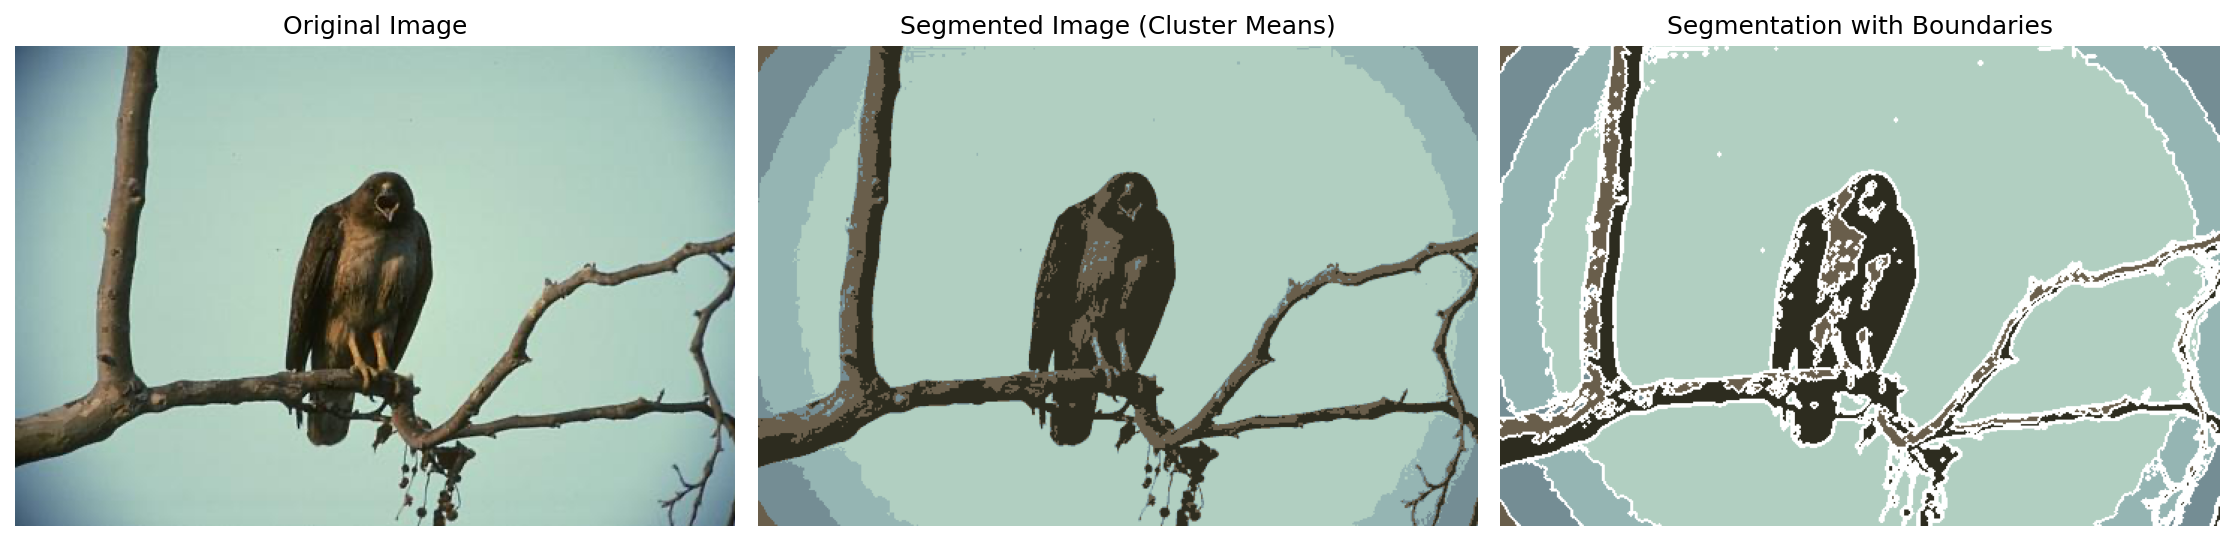
\includegraphics[width=0.9\textwidth]{part5/results/part5a_segmentation_k5.png}
\caption{K-means segmentation with $k=5$ clusters: original (left), segmented with cluster means (center), boundaries highlighted (right)}
\end{figure}

The k-means algorithm converged after multiple iterations, successfully grouping pixels into five perceptually distinct color regions. The segmentation captures major color variations in the image, with each cluster representing a coherent region.

\textbf{Final cluster statistics:}
\begin{itemize}
    \item The algorithm achieved convergence with mean shifts below $10^{-4}$
    \item Cluster sizes vary based on the prevalence of each color in the image
    \item Cluster means represent the average RGB values of each segment
\end{itemize}

\textbf{Observations:}
\begin{itemize}
    \item K-means produces regions of uniform color, effectively simplifying the image
    \item Boundaries follow color discontinuities but ignore spatial coherence
    \item The method treats each pixel independently, potentially creating fragmented regions
    \item Computational complexity is $O(nk)$ per iteration for $n$ pixels and $k$ clusters
\end{itemize}

\subsection{Part (b): SLIC Superpixels }

\subsubsection{Overview}
Simple Linear Iterative Clustering (SLIC) extends k-means to produce spatially coherent superpixels. Unlike standard k-means, SLIC incorporates spatial proximity alongside color similarity, ensuring compact, roughly uniform regions.

\subsubsection{Color Space and Features}
SLIC operates in CIELAB color space, which is perceptually uniform (equal distances correspond to equal perceptual differences). Each pixel is represented by a 5D feature vector:
$\mathbf{f}_i = [L_i, a_i, b_i, x_i, y_i]^T$

where $(L, a, b)$ are CIELAB color coordinates and $(x, y)$ are spatial coordinates.

The RGB to LAB conversion involves:
\begin{enumerate}
    \item Convert RGB to linear RGB via gamma correction
    \item Transform to CIE XYZ using standard illuminant D65
    \item Apply the nonlinear LAB transformation:
    $L = 116f(Y/Y_n) - 16, \quad a = 500[f(X/X_n) - f(Y/Y_n)], \quad b = 200[f(Y/Y_n) - f(Z/Z_n)]$
    where $f(t) = t^{1/3}$ for $t > (6/29)^3$
\end{enumerate}

\subsubsection{Distance Metric}
SLIC uses a combined distance that balances color and spatial proximity:
$D = \sqrt{\left(\frac{d_{\text{lab}}}{m}\right)^2 + \left(\frac{d_{xy}}{s}\right)^2}$

where:
\begin{itemize}
    \item $d_{\text{lab}} = \sqrt{(L_i - L_j)^2 + (a_i - a_j)^2 + (b_i - b_j)^2}$ is color distance
    \item $d_{xy} = \sqrt{(x_i - x_j)^2 + (y_i - y_j)^2}$ is spatial distance
    \item $s$ is the nominal superpixel spacing (grid step size)
    \item $m$ is a compactness parameter controlling the color-space trade-off
\end{itemize}

The parameter $m = 10$ emphasizes spatial regularity, producing compact superpixels. Larger $m$ creates more irregular shapes that better follow color boundaries.

\subsubsection{Algorithm}
SLIC initializes $k$ cluster centers on a regular grid with spacing $s = \sqrt{N/k}$ pixels, then iteratively refines them:

\textbf{Initialization:}
\begin{enumerate}
    \item Place centers at grid positions spaced by $s$ pixels
    \item Perturb each center to the lowest gradient location in a $3 \times 3$ neighborhood
\end{enumerate}

The perturbation step moves centers away from edges, improving stability.

\textbf{Iteration:}
\begin{enumerate}
    \item \textbf{Assignment:} For each center, search only in a $2s \times 2s$ region (efficient!)
    \item Assign each pixel to the nearest center using distance $D$
    \item \textbf{Update:} Recompute centers as the mean of assigned pixels
    \item Check convergence: stop if center shifts are below threshold
\end{enumerate}

\textbf{Post-processing:}
Enforce connectivity by merging small isolated components (< 10 pixels) into adjacent superpixels using a breadth-first search.

\subsubsection{Computational Complexity}
SLIC is remarkably efficient: $O(n)$ per iteration since each pixel only compares to nearby centers ($O(1)$ comparisons), unlike k-means which requires $O(k)$ comparisons per pixel.

\subsubsection{Results}

\begin{figure}[H]
\centering
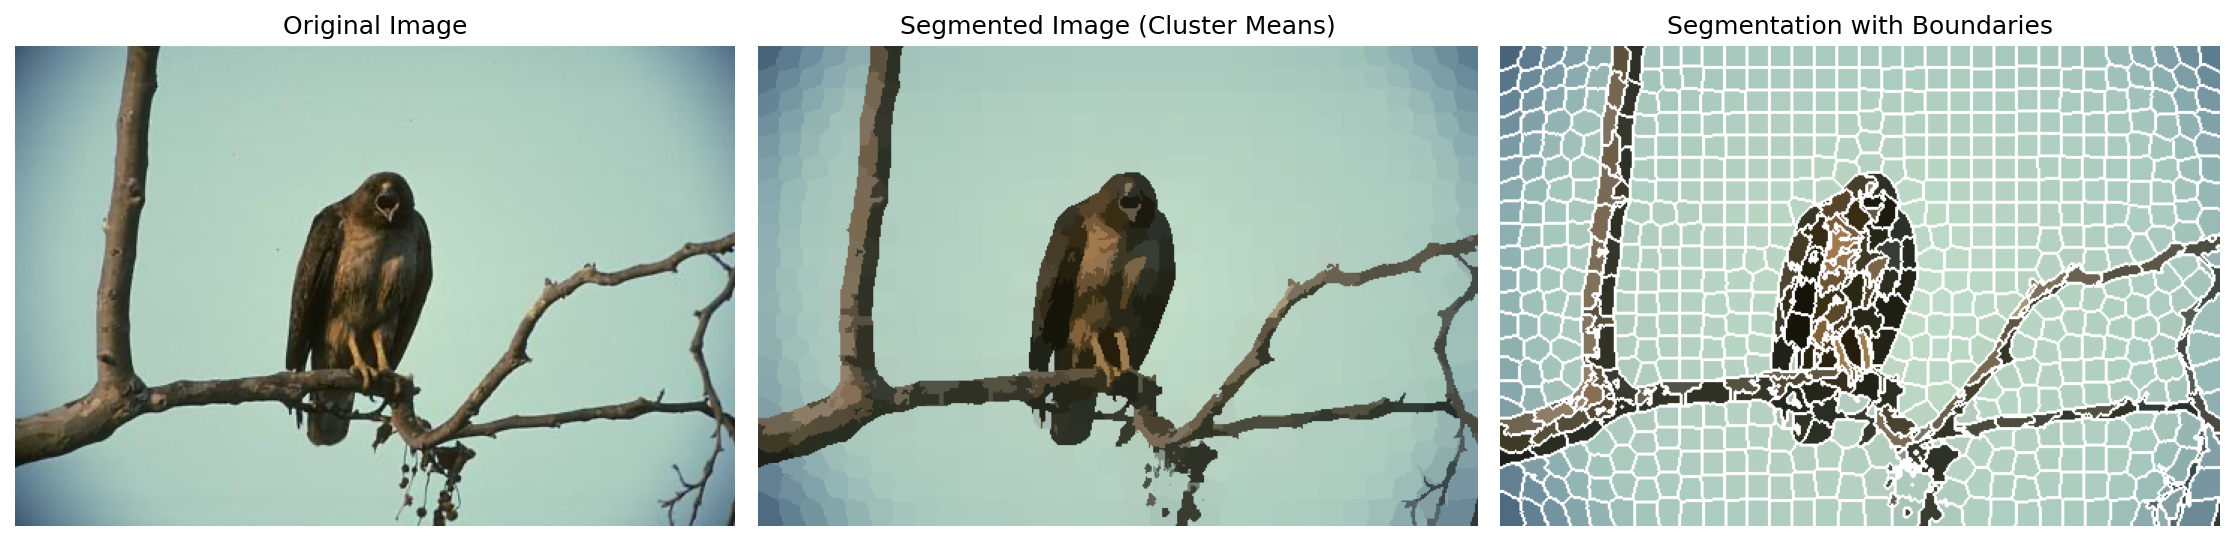
\includegraphics[width=0.9\textwidth]{part5/results/part5b_slic_s15_m10.png}
\caption{SLIC superpixels with $s=15$, $m=10$: original (left), superpixel means (center), boundaries (right)}
\end{figure}

SLIC successfully generates compact, approximately uniform superpixels with the following characteristics:
\begin{itemize}
    \item Superpixel spacing $s = 15$ pixels produces hundreds of regions
    \item Average superpixel size: $\sim s^2 = 225$ pixels
    \item Boundaries align well with image edges while maintaining spatial regularity
    \item The algorithm converged in approximately 10 iterations
\end{itemize}

\textbf{Comparison with k-means:}
\begin{itemize}
    \item SLIC produces spatially coherent regions; k-means produces fragmented regions
    \item SLIC boundaries respect both color and spatial continuity
    \item SLIC is much faster due to localized search
    \item Superpixels are more suitable as primitives for higher-level segmentation algorithms
\end{itemize}

\subsection{Part (c): Graph Cut Segmentation (Optional)}

\subsubsection{Overview}
Graph cut segmentation formulates the problem as energy minimization on a graph, where pixels are nodes and edges encode similarity. The goal is to partition the graph into foreground and background regions that minimize a global energy function.

\subsubsection{Graph Construction}
We construct a graph $G = (V, E)$ with $|V| = n + 2$ vertices:
\begin{itemize}
    \item $n$ vertices for image pixels
    \item 2 special vertices: source $s$ (foreground) and sink $t$ (background)
\end{itemize}

Edges have capacities representing the cost of cutting them:

\textbf{Terminal edges (region costs):}
Connect each pixel $p$ to source and sink:
$c(s, p) = -\log P(I_p | \text{foreground}), \quad c(p, t) = -\log P(I_p | \text{background})$

For known foreground/background pixels (user-specified rectangles), we set infinite capacity to enforce hard constraints.

\textbf{Neighbor edges (boundary costs):}
Connect 4-adjacent pixels with capacity encoding color similarity:
$c(p, q) = \lambda \exp\left(-\frac{\|I_p - I_q\|^2}{2\sigma^2}\right)$

High capacity (similar colors) means high cost to separate, encouraging smooth boundaries. The parameter $\lambda = 100$ controls the smoothness penalty.

\subsubsection{Energy Minimization}
The segmentation corresponds to an $s$-$t$ cut: a partition of vertices into sets $S$ (containing $s$) and $T$ (containing $t$). The cut's cost is:
$E(S, T) = \sum_{p \in S, q \in T} c(p, q)$

By the max-flow min-cut theorem, the minimum cut equals the maximum flow from $s$ to $t$. The Ford-Fulkerson or push-relabel algorithms compute this efficiently.

\subsubsection{Likelihood Models}
Color likelihoods are estimated from user-provided foreground and background samples:
$P(I_p | \text{foreground}) \propto \exp\left(-\frac{\|I_p - \mu_{\text{fg}}\|^2}{2\sigma_{\text{fg}}^2}\right)$

where $\mu_{\text{fg}}$ is the mean color of foreground samples. A similar model applies to background.

\subsubsection{Implementation Details}
\begin{enumerate}
    \item Define foreground rectangle (center region) and background rectangle (corner region)
    \item Build sparse capacity matrix with $n+2$ vertices
    \item Set terminal capacities based on color models and constraints
    \item Set neighbor capacities based on color similarity
    \item Compute maximum flow using SciPy's \texttt{maximum\_flow}
    \item Extract cut from residual graph via breadth-first search from source
\end{enumerate}

For computational efficiency, the image was resized to $300 \times 300$ pixels before processing.

\subsubsection{Results}

\begin{figure}[H]
\centering
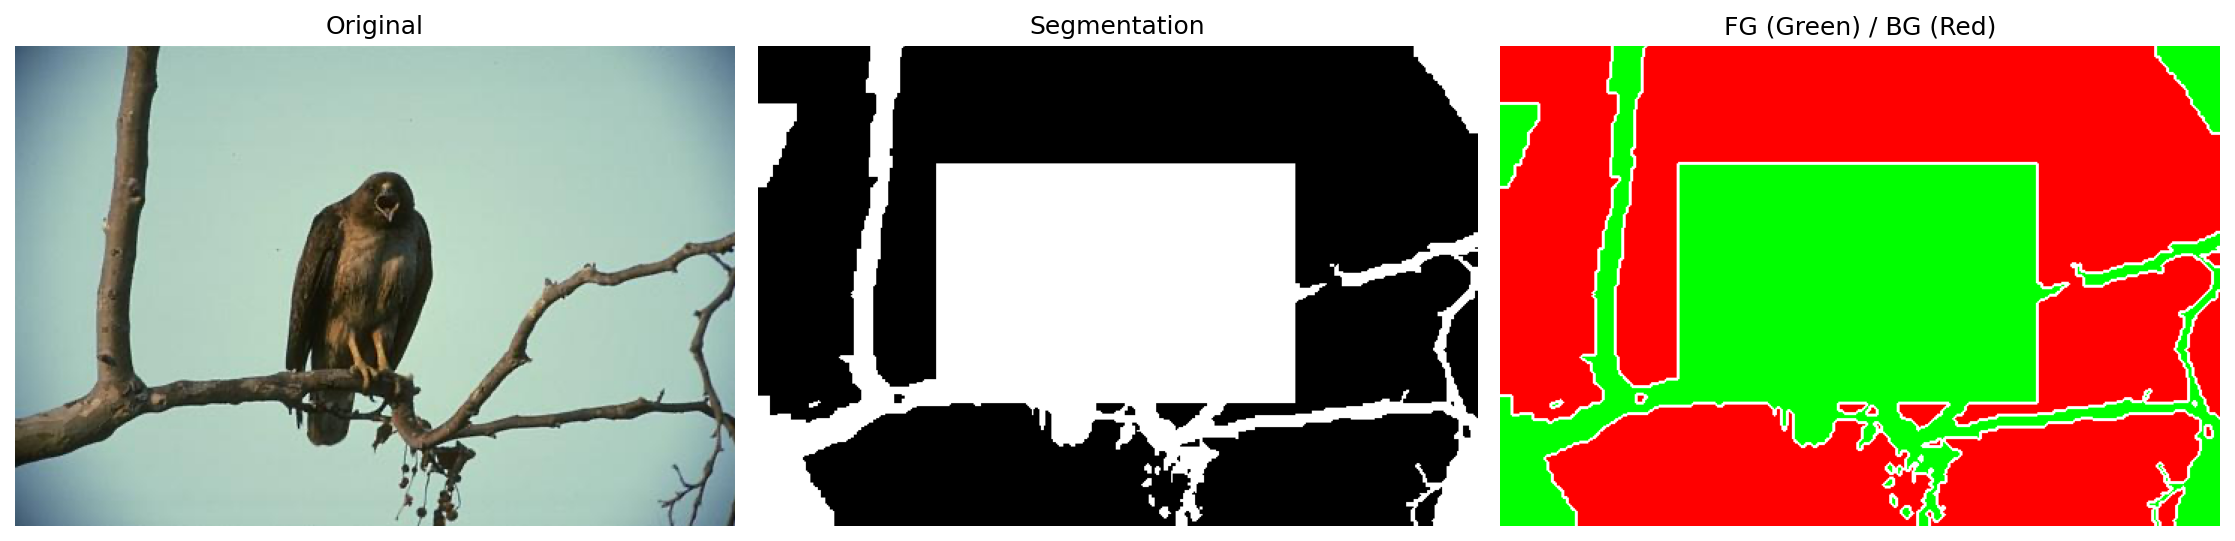
\includegraphics[width=0.9\textwidth]{part5/results/part5c_graphcut.png}
\caption{Graph cut segmentation: original (left), binary mask (center), colored result with foreground (green) and background (red) separated by white boundary (right)}
\end{figure}

The graph cut algorithm successfully separates foreground from background based on the color models derived from sample regions. The segmentation boundary follows color discontinuities while maintaining global coherence.

\textbf{Performance characteristics:}
\begin{itemize}
    \item Foreground and background regions are well-separated
    \item The boundary is smoother than k-means due to the spatial smoothness term
    \item The method is sensitive to the choice of sample regions
    \item Maximum flow computation scales to moderate image sizes (\< 500 pixels)
\end{itemize}

\textbf{Advantages of graph cuts:}
\begin{itemize}
    \item Global optimality: finds the minimum cut exactly
    \item Incorporates both region and boundary information
    \item Handles user constraints naturally via terminal capacities
    \item Produces coherent segmentation with smooth boundaries
\end{itemize}

\subsection{Part (d): Watershed Segmentation }

\subsubsection{Overview}
Watershed segmentation treats the gradient magnitude image as a topographic surface: intensity represents elevation, and the algorithm finds the "watersheds" (ridges) separating catchment basins (valleys).

\subsubsection{Gradient Computation}
We compute the gradient magnitude across all three RGB channels and combine them:
$|\nabla I| = \sqrt{\frac{1}{3}\sum_{c \in \{R,G,B\}} |\nabla I_c|^2}$

This RMS gradient captures color edges that may not be visible in any single channel. Sobel operators are used for the spatial derivatives in each channel.

\subsubsection{Preprocessing}
Two filtering steps improve watershed quality:

\textbf{Gaussian smoothing:} Before gradient computation, smooth the image with $\sigma = 2$ to reduce noise:
$I_{\text{smooth}} = I * G_\sigma$

This prevents over-segmentation from texture and noise.

\textbf{H-minima transform:} Suppress shallow minima in the gradient image:
$H_h(f)(x) = \max\{f(x), \min_{y \in \Omega} [f(y) + h \cdot d(x,y)]\}$

where $d(x,y)$ is distance. In practice, we use the simpler formulation:
$f_h = \min(f + h, 255)$

This eliminates small local minima while preserving deep minima at significant region boundaries. The parameter $h = 10$ was chosen to suppress texture while retaining major edges.

\subsubsection{Watershed Algorithm}
The immersion simulation algorithm:

\begin{enumerate}
    \item \textbf{Find regional minima:} Identify connected components of pixels that are local minima of the gradient
    \item \textbf{Label minima:} Assign each minimum region a unique label
    \item \textbf{Flooding simulation:} Sort all unlabeled pixels by gradient value
    \item Process pixels in increasing gradient order:
    \begin{itemize}
        \item If pixel has labeled neighbors from exactly one basin: assign to that basin
        \item If pixel has labeled neighbors from multiple basins: mark as watershed line
    \end{itemize}
\end{enumerate}

This simulates water flooding the topographic surface from the minima. Watersheds form where different basins meet.

\subsubsection{Results}

\begin{figure}[H]
\centering
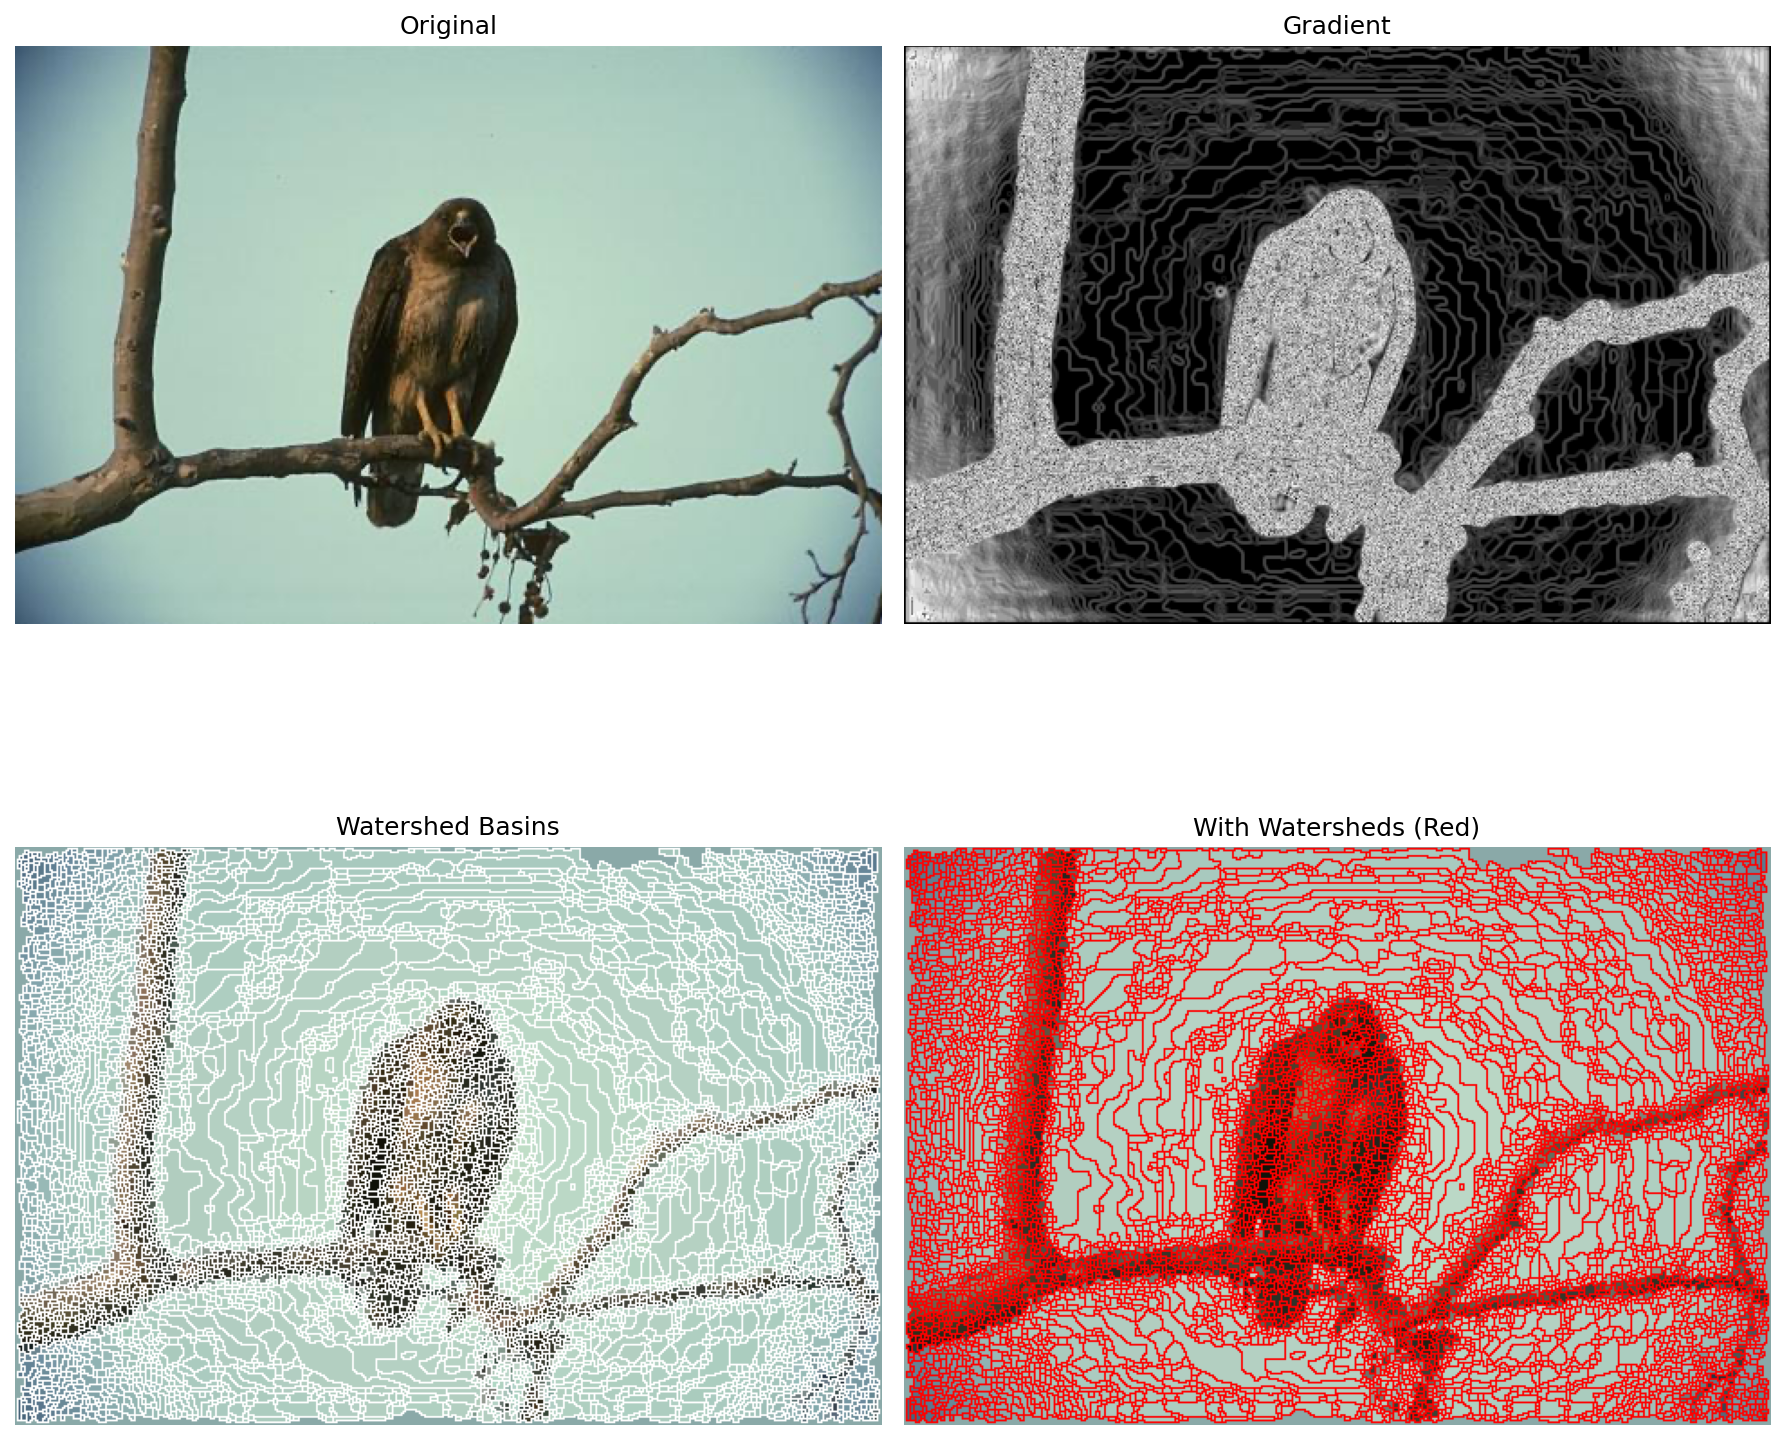
\includegraphics[width=0.9\textwidth]{part5/results/part5d_watershed_h10.png}
\caption{Watershed segmentation: original (top left), gradient magnitude (top right), watershed basins colored by mean (bottom left), basins with watershed lines in red (bottom right)}
\end{figure}

The watershed algorithm segments the image into numerous regions, each corresponding to a local intensity valley. The gradient image shows strong responses at color boundaries, and the watershed lines accurately follow these edges.

\textbf{Observations:}
\begin{itemize}
    \item H-minima parameter $h = 10$ controls segmentation granularity
    \item Without h-minima suppression, severe over-segmentation occurs (thousands of tiny regions)
    \item Watershed lines (red) mark boundaries between catchment basins
    \item Each basin is colored by its mean RGB value for visualization
    \item The number of basins depends on the gradient structure and h-minima threshold
\end{itemize}

\textbf{Comparison with other methods:}
\begin{itemize}
    \item Watershed produces more regions than k-means, following local intensity structure
    \item Unlike SLIC, watersheds have irregular sizes adapted to gradient topology
    \item Boundaries are more accurate than k-means but potentially more fragmented
    \item The method is purely local (no global optimization like graph cuts)
\end{itemize}

\subsection{Comparative Discussion}

The four segmentation methods represent different philosophical approaches:

\textbf{K-means:} Pure color clustering without spatial constraints. Fast and simple but produces fragmented regions. Best for color quantization or when spatial coherence is unimportant.

\textbf{SLIC:} Balanced color and spatial clustering producing uniform superpixels. Excellent preprocessing for higher-level algorithms. Combines efficiency with good boundary adherence.

\textbf{Graph cuts:} Global energy minimization with explicit boundary and region terms. Produces coherent segmentations but requires user input and significant computation. Best for interactive segmentation with foreground/background specification.

\textbf{Watershed:} Region growing based on gradient topology. Sensitive to noise but captures fine detail when properly preprocessed. Best for images with clear intensity boundaries.

Each method has optimal use cases depending on application requirements: computational budget, need for user interaction, desired segmentation granularity, and importance of spatial coherence versus color accuracy.

\end{document}